\documentclass[]{hdsr}
\begin{document}
\begin{center}

  \title{Método de convergencia acelerada \Delta^2  Aitken}
  \maketitle
  \thispagestyle{empty}
  
  
  % Authors and Affiliations
  \begin{tabular}{cc}
    Pedro Guerrero, Carlos Erazo , María Alejandra Sandoval, Valentina Rozo \\[0.20ex]
  \end{tabular}
  \date{\today}
\end{center}

\hspace{10pt}
  \small	
\copyrightnotice

\section*{Método de Aitken}
El método de Aitken usado por Alexander Aitken en 1926, se utiliza acelerar la convergencia de una secuencia que es linealmente convergente, independientemente de su origen[2]. Es decir, encuentra en un menor número de iteraciones el número al que converge comparado con otros métodos. Este algoritmo fue mejorado de tal manera que hace que una secuencia dada por el método de punto fijo converja de forma más rápida, este método se denomina, método de Steffensen. La fórmula de Aitken es:

\begin{equation}
    {Pn} = {Pn}-\frac{\((Pn+1 - Pn)^2}{(Pn+2 - 2Pn+1 + Pn)}
\end{equation}

\section*{Método de Steffensen}
El método Steffensen es un algoritmo para obtener la raíz de la función, este método es considerado una combinación entre el método de punto fijo y el método de Aitken; este algoritmo presenta una convergencia cuadrática, además de presentar una convergencia hacia la raíz. La fórmula de Steffensen es:

\begin{equation}
    {Xn+1} = {Xn}-\frac{\((g(Xn)-Xn)^2}{g(g(Xn))-2g(Xn)+Xn}
\end{equation}
\section{Solución}
\label{sec1}
\subsection{Condiciones iniciales}
Para este caso en particular se va observar el funcionamiento del método de Aitken desde el método de Steffensen. Las condiciones necesarias para implementar el algoritmo son las siguientes:\newline

- Se debe definir el intervalo en el que se va a evaluar.\newline

- Se debe definir la tolerancia.\newline

- Se debe definir el valor inicial.\newline

- Debe ser continua.\newline

- Debe estar cerca de una raíz.\newline

- Se espera que la función converja en este intervalo, sin embargo la implementación tiene en cuenta los puntos donde esto es un problema. \newline

- Casos como división por cero al momento de evaluar el algoritmo también se tienen en cuenta. \newline

El algoritmo se va a evaluar con las siguientes funciones:\newline

\begin{equation}
    {F(x)} = cos^2(2x)-x^2
\end{equation}
\begin{equation}
    {F(x)} = xsin(x)-1,     x = [-1, 2]
\end{equation}
\begin{equation}
    {F(x)} = x^3 -2x^2 + \frac{4}{3}x - \frac{8}{27}
\end{equation}

\section{Diagrama de flujo}
\begin{center}
  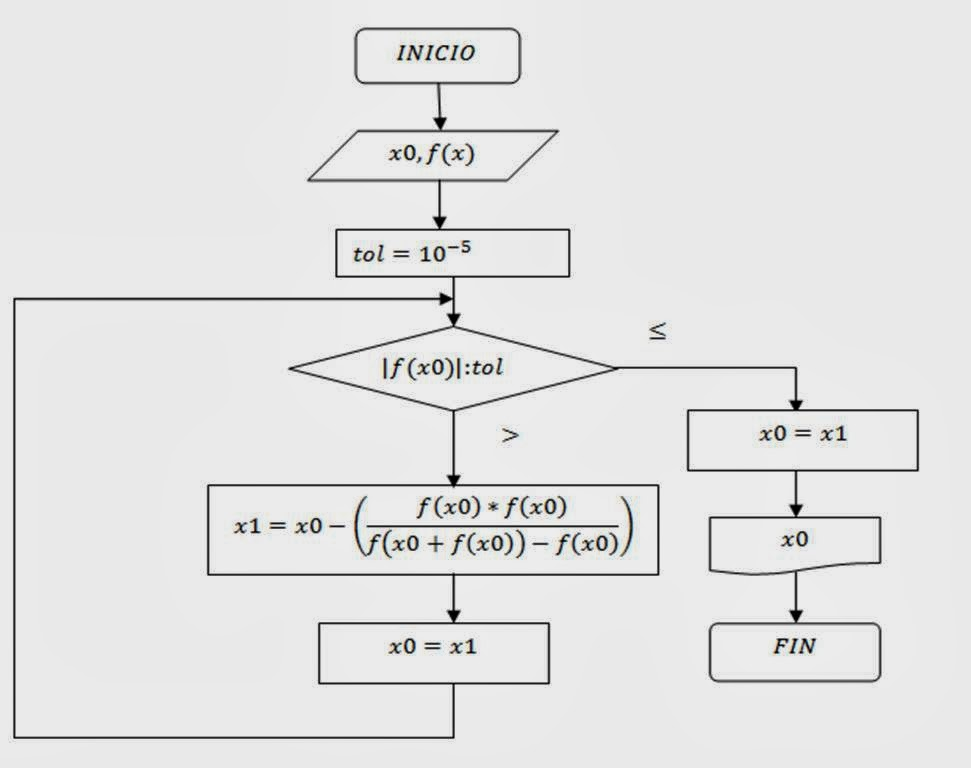
\includegraphics[width=\textwidth]{figs/steffensen03.jpg} 
  \begin{figure}[H]
    \centering
    \includegraphics[scale=0.35]{iris_pairs} \\
    \caption{Diagrama de flujo del método Steffensen [1]}
    \label{fig:my_label}
\end{figure}
\end{center}

Para la implementación del método de Steffensen, se toma como referencia la Figura 1. La cual describe el funcionamiento del método para un caso general, comenzando con una función, un punto inicial y una tolerancia (que puede tomar cualquier valor) después de esto comienza un ciclo donde se busca constantemente que al evaluar este punto inicial el resultado se encuentre dentro de la tolerancia especificada, de no ser así se evalúa en la ecuación (0.2) y se remplaza el valor del punto inicial que se evalúa nuevamente. Cuando el resultado esta dentro de la tolerancia establecida se retorna su valor. \newline

\section{Análisis}
\subsection{Resultados}
Los resultados de las raíces para las funciones se validan al evaluar cada función en ese resultado, si el resultado de la función se aproxima a cero, quiere decir que ese resultado corresponde al valor de la raíz; a continuación se muestran los resultados de las raíces para cada función:\newline

- Para la función de coseno, el resultado de la raíz es 0.514933264661 con un total de 4 y 5 iteraciones con su mínima y máxima tolerancia respectivamente, al evaluarlo en la función el resultado es 0,0. \newline

- Para la función de seno, el resultado de la raíz es 1.11415714087 con un total de  3 y 4 iteraciones con su mínima y máxima tolerancia respectivamente, al evaluarlo en la función el resultado es 0,0. \newline

- Para la función del polinomio, el resultado de la raíz es 0.666295955891 con un total de  15 y 31 iteraciones con su mínima y máxima tolerancia respectivamente, al evaluarlo en la función el resultado es del orden de e-11. \newline

\subsection{Comportamiento}\newline
Teniendo en cuenta los riesgos a los que una implementación de este tipo esta expuesta se toman las siguientes medidas para cada caso y en algunas se presentan los siguientes resultados. \newline

1)Pérdida de significancia.\newline

2)Número de iteraciones.\newline

3)Convergencia.\newline


-Para la función de coseno no se presenta pérdida de significancia, el numero de iteraciones es menor con respecto al método de bisección, con un total de 4 y 5 iteraciones en sus tolerancias. La función es convergente ya que dentro del intervalo presenta una sola raíz.\newline


-Para la función de seno no se presenta pérdida de significancia, el número de iteraciones es menor con respecto al método de bisección, con un total de  3 y 4 iteraciones en sus tolerancias. La función es divergente ya que dentro del intervalo presenta más de una raíz, pero cuando se definen otros intervalos la función converge.\newline


-Para la función del polinomio no se presenta pérdida de significancia, el número de iteraciones es menores con respecto al método de bisección, con un total de  15 y 31 iteraciones en sus tolerancias. La función es convergente  ya que dentro del intervalo presenta una sola raíz. 

Con respecto al algoritmo de bisección, el algoritmo de Steffensen se comporta de una manera más eficiente al realizar menos iteraciones con todas las funciones evaluadas en todas las tolerancias.

\subsection{Soluciones a problemas}\newline
Para solucionar el problema de la significancia se puede usar el tipo de dato float128 de la librería "Numpy", con el fin de que las cifras significativas aumenten al número que se desea y no el que se encuentra predeterminado en el programa. De este modo los niveles de tolerancia pueden ser más grandes con el fin de que la diferencia entre los valores sea lo más exactos posible. Para acceder a estos valores en la implementación para acceder al valor completo se usa la librería "Decimal".

\subsection{Preguntas importantes}
-¿Qué pasa con el método cuando hay dos raíces?

Cuando se presentan dos raíces en el método este diverge en vez de converger, debido a que no sabe a cuál de las dos raíces debe acercarse. Para evitar esto la implementación identifica los puntos donde la función diverge y los omite, dado que este no es el objetivo, para los demás valores se retorna el resultado de la raíz más cercana.\newline

-¿Qué pasa con el método cuando la función es periódica, par o impar, estas características influyen?

Si una función es par significa que f(x) = f(-x), si una función es impar significa que f(x) != f(-x) en el caso particular del método que implementamos no influye que la función sea par o impar, debido a que el método va a encontrar las raíces indistintamente; pero si la función es par se van a obtener los mismos resultados al evaluar la parte positiva como la parte negativa. Cuando la función es periódica, el método de igual forma cumple con su objetivo, pero sus resultados se pueden ver afectados ya que el método puede retornar valores para raíces próximas o anteriores.\newline


    \subsection{Gráficas resultados Steffensen}
    \begin{center}
        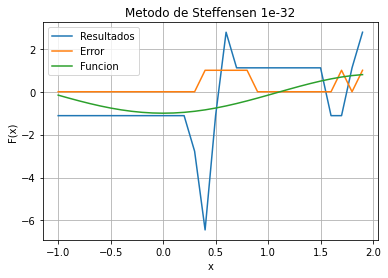
\includegraphics[width=0.7\textwidth]{figs/sen(-32).png} 
        \begin{figure}[H]
            \centering
            \caption{}
            \label{fig:my_label}
            Resultados función x(sen(x)-1 aplicada con el método Steffensen\\
        \end{figure}
    \end{center}
    
    \begin{center}
        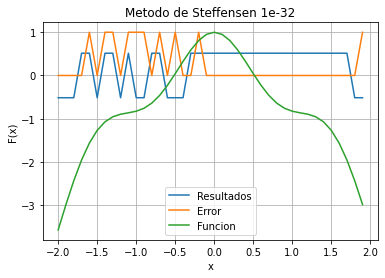
\includegraphics[width=0.7\textwidth]{figs/cos(-32).png} 
        \begin{figure}[H]
            \centering
            \caption{}
            \label{fig:my_label}
            Resultados función \text{cos^2(2x)-x^2} \\\hspace{0.2cm} aplicada con el método Steffensen\\
        \end{figure}
    \end{center}
    
    \begin{center}
        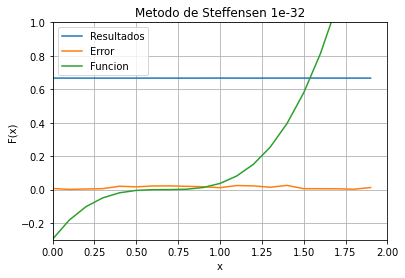
\includegraphics[width=0.7\textwidth]{figs/polzoom.png} 
        \begin{figure}[H]
            \centering
            \caption{}
            \label{fig:my_label}
            Resultados función \text{x^3-2x^2+(4/3)x-(8/27)}\\\hspace{0.2cm} aplicada con el método de Steffensen\\
        \end{figure}
    \end{center}
    
    Al realizar la implementación en cada una de las funciones, da como resultado la Figura 2, 3 y 4, donde se evidencia en primer lugar, la función, sus resultados y el error en el intervalo que se trató. Este error se toma teniendo en cuenta el punto i e i+1 de los resultados.
    \hfill
    \hspace{5pt}
            
                
                    
                   
    
    
    \subsection{Gráficas Bisección vs Steffensen}
    
    \begin{center}
        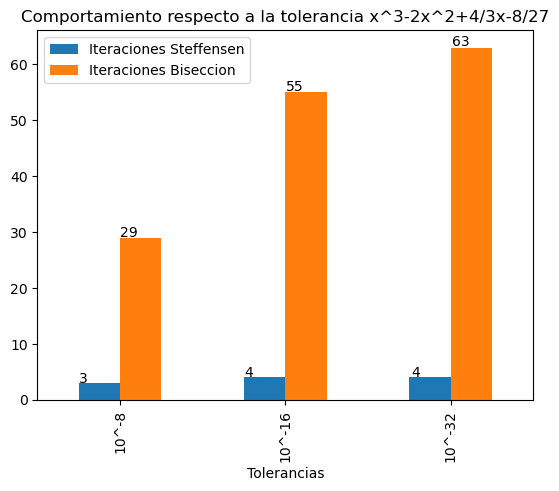
\includegraphics[width=0.6\textwidth]{figs/seno.png} 
        \begin{figure}[h]
            \centering
            \caption{}
            \label{fig:my_label5}
            Comportamiento del número de iteraciones en bisección y Steffensen respecto a la tolerancia de la función x(sen(x))-1\\
        \end{figure}
    \end{center}
    \hfill
    
    \begin{center}
        \begin{figure}[h]
            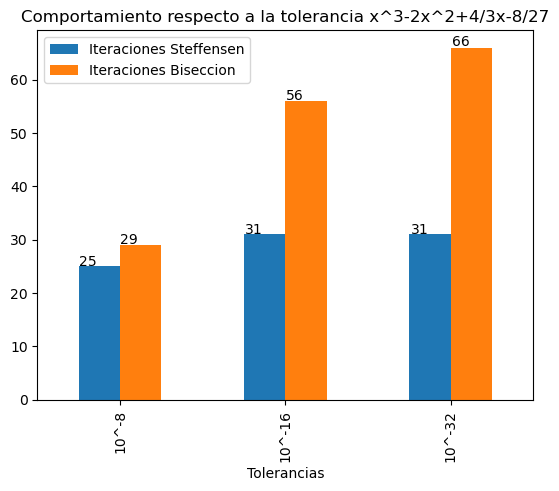
\includegraphics[width=0.6\textwidth]{figs/polinomio.png} 
            \caption{}
            \label{fig:my_label7}
            Comportamiento del número de iteraciones en bisección y Steffensen respecto a la tolerancia de la función \text{(x^3)-2x^2+(4/3)x-(8/27))}\\
        \end{figure}
    \end{center}
    \hfill
    
    
     \begin{center}
        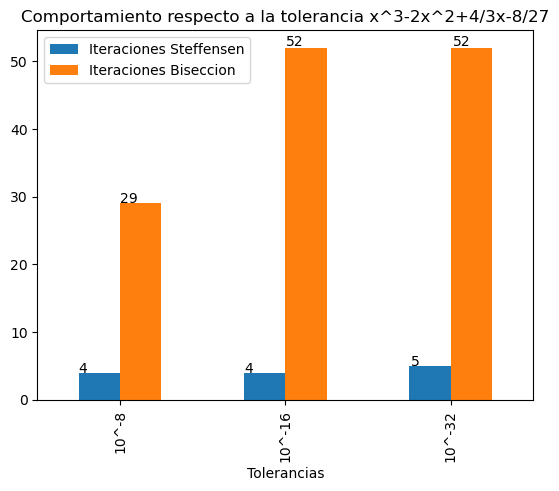
\includegraphics[width=0.6\textwidth]{figs/coseno.png} 
        \begin{figure}[h]
            \centering
            \caption{}
            \label{fig:my_label6}
            Comportamiento del número de iteraciones en bisección y Steffensen respecto a la tolerancia de la función \text{cos^2(2x)-(x^2)}\\
        \end{figure}
    \end{center}
    \hfill
    
        
    Las figuras 5, 6 y 7, corresponden a la comparación entre el método de bisección y el método de Steffensen en cada una de las funciones. Se puede observar que al evaluar los puntos dentro del mismo rango, Steffensen converge de manera más rápida, dejando ver que el método de bisección no es eficiente frente el numero de iteraciones realizadas para entregar un resultado.

\section{Referencias}

[1] A. Guillén, «wordpress,» Arturo Guillén Informática-UCR, [En línea]. \newline
Available: https://arturoguillen90.wordpress.com/aceleracion-de-convergencia/steffensen/. [Último acceso: 31 08 2020].

[2] R. L. Burden y J. D. F. , «uvirtual,» 2011. [En línea].\newline Available: https://uvirtual.javeriana.edu.co/bbcswebdav/pid-486752-dt-content-rid-3640392_1\newline/courses/001291_2030_1039/analisis_numerico_burden.pdf. [Último acceso: 31 08 2020].
\end{document}


